% Practice Test 16 — Oklahoma Edition
% Questions: 30 (19 MC + 11 SA)
% Generated by scripts/generate_practice_tests.py

\begin{practiceQuestion}{1-3-q24}{sa}
\begin{questionText}
The table shows a proportional relationship. Find $k$ and the missing value.

\begin{center}
\begin{tabular}{|c|c|}
\hline $x$ & $y$ \\ \hline $3$ & $7.5$ \\ $?$ & $15$ \\ $10$ & $25$ \\ \hline
\end{tabular}
\end{center}
\end{questionText}
\correctAnswer{$k = 2.5$; missing $x = 6$}
\explanation{$k = \frac{7.5}{3} = 2.5$. For the missing row: $15 = 2.5x$ so $x = 15 \div 2.5 = 6$.}
\end{practiceQuestion}

\begin{practiceQuestion}{1-6-q27}{gmc}
\begin{questionText}
A map uses the scale shown below. If two cities are $6.5$ cm apart on the map, what is the actual distance?

\begin{center}
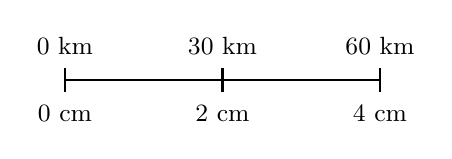
\begin{tikzpicture}[scale=1]
  \draw[thick] (0,0) -- (4,0);
  \draw[thick] (0,-0.15) -- (0,0.15);
  \draw[thick] (2,-0.15) -- (2,0.15);
  \draw[thick] (4,-0.15) -- (4,0.15);
  \node[below] at (0,-0.2) {\small $0$ cm};
  \node[below] at (2,-0.2) {\small $2$ cm};
  \node[below] at (4,-0.2) {\small $4$ cm};
  \node[above] at (0,0.2) {\small $0$ km};
  \node[above] at (2,0.2) {\small $30$ km};
  \node[above] at (4,0.2) {\small $60$ km};
\end{tikzpicture}
\end{center}
\end{questionText}
\choiceA{$90$ km}
\choiceB{$95$ km}
\choiceC{$97.5$ km}
\choiceD{$100$ km}
\correctAnswer{C}
\explanation{Scale: $2$ cm $= 30$ km, so $1$ cm $= 15$ km. For $6.5$ cm: $15 \times 6.5 = 97.5$ km.}
\end{practiceQuestion}

\begin{practiceQuestion}{1-7-q28}{gmc}
\begin{questionText}
The table below shows the model and actual measurements of different objects. Which object has the largest scale factor?

\begin{center}
\begin{tabular}{|l|c|c|}
\hline
\textbf{Object} & \textbf{Model} & \textbf{Actual} \\
\hline
Car & $10$ cm & $5$ m \\
\hline
Boat & $8$ cm & $24$ m \\
\hline
House & $12$ cm & $6$ m \\
\hline
\end{tabular}
\end{center}
\end{questionText}
\choiceA{Car}
\choiceB{Boat}
\choiceC{House}
\choiceD{Car and House (tied)}
\correctAnswer{B}
\explanation{Car: $500 \div 10 = 50$. Boat: $2{,}400 \div 8 = 300$. House: $600 \div 12 = 50$. The boat has the largest scale factor ($1 : 300$).}
\end{practiceQuestion}

\begin{practiceQuestion}{2-1-q07}{mc}
\begin{questionText}
A store has $300$ items in stock. If $60\%$ are on sale, how many items are on sale?
\end{questionText}
\choiceA{$120$}
\choiceB{$150$}
\choiceC{$180$}
\choiceD{$200$}
\correctAnswer{C}
\explanation{$60\% = 0.60$. Multiply: $0.60 \times 300 = 180$ items.}
\end{practiceQuestion}

\begin{practiceQuestion}{2-4-q28}{gmc}
\begin{questionText}
The bar model below shows the breakdown of a customer's total payment. What was the original price of the item before the sales tax?

\begin{center}
\begin{tikzpicture}[scale=0.65]
  \fill[funBlue!40] (0,0) rectangle (9,1);
  \fill[funRed!40] (9,0) rectangle (10,1);
  \draw[thick] (0,0) rectangle (10,1);
  \draw[thick] (9,0) -- (9,1);
  \node[font=\small] at (4.5,0.5) {Original price};
  \node[font=\small] at (9.5,0.5) {Tax};
  \draw[thick,<->] (0,-0.4) -- (10,-0.4) node[midway,below,font=\small] {Total $= \$53.50$};
  \node[above,font=\small] at (9.5,1) {$7\%$};
\end{tikzpicture}
\end{center}
\end{questionText}
\choiceA{$\$46.76$}
\choiceB{$\$49.76$}
\choiceC{$\$50.00$}
\choiceD{$\$52.00$}
\correctAnswer{C}
\explanation{The total is $1.07$ times the original. Original $= 53.50 \div 1.07 = \$50.00$.}
\end{practiceQuestion}

\begin{practiceQuestion}{2-7-q25}{sa}
\begin{questionText}
A jogger estimated running $5$ miles but actually ran $4.8$ miles. What is the percent error (rounded to the nearest tenth)?
\end{questionText}
\correctAnswer{$\approx 4.2\%$}
\explanation{$\frac{|5 - 4.8|}{4.8} \times 100 = \frac{0.2}{4.8} \times 100 \approx 4.17 \approx 4.2\%$.}
\end{practiceQuestion}

\begin{practiceQuestion}{2-8-q27}{gmc}
\begin{questionText}
The table below shows the monthly fees at four financial institutions. Which institution has the lowest annual fee?

\begin{center}
\begin{tabular}{|l|c|}
\hline
\textbf{Institution} & \textbf{Monthly Fee} \\
\hline
Big Bank & $\$8$ \\
\hline
Town Credit Union & $\$2$ \\
\hline
City Bank & $\$5$ \\
\hline
Online Bank & $\$0$ \\
\hline
\end{tabular}
\end{center}
\end{questionText}
\choiceA{Big Bank}
\choiceB{Town Credit Union}
\choiceC{City Bank}
\choiceD{Online Bank}
\correctAnswer{D}
\explanation{Online Bank charges $\$0$/month, so the annual fee is $\$0$. That is the lowest.}
\end{practiceQuestion}

\begin{practiceQuestion}{3-1-q10}{mc}
\begin{questionText}
A football team gains $8$ yards on one play and loses $8$ yards on the next play. What is the net result?
\end{questionText}
\choiceA{$16$ yards gained}
\choiceB{$8$ yards gained}
\choiceC{$8$ yards lost}
\choiceD{$0$ yards}
\correctAnswer{D}
\explanation{$8 + (-8) = 0$. Gaining and losing the same amount are opposite actions that cancel out.}
\end{practiceQuestion}

\begin{practiceQuestion}{4-1-q22}{sa}
\begin{questionText}
Evaluate $\frac{x^2 - 1}{4}$ when $x = 5$.
\end{questionText}
\correctAnswer{$6$}
\explanation{Substitute: $\frac{5^2 - 1}{4} = \frac{25 - 1}{4} = \frac{24}{4} = 6$.}
\end{practiceQuestion}

\begin{practiceQuestion}{4-2-q20}{sa}
\begin{questionText}
Simplify $\frac{1}{2}x + \frac{3}{4}x - 2$.


\begin{center}
\fractionCircle{1}{2}
\hspace{1cm}
\fractionCircle{3}{4}
\end{center}
\end{questionText}
\correctAnswer{$\frac{5}{4}x - 2$ or $1\frac{1}{4}x - 2$}
\explanation{Find a common denominator: $\frac{2}{4}x + \frac{3}{4}x = \frac{5}{4}x$. The constant stays: $\frac{5}{4}x - 2$.}
\end{practiceQuestion}

\begin{practiceQuestion}{5-3-q28}{gmc}
\begin{questionText}
Look at the number line. The expression $3(x + 2)$ equals the distance from $A$ to $B$. What is $x$?

\begin{center}
\begin{tikzpicture}[scale=0.6]
  \draw[thick,->] (-1,0) -- (16,0);
  \foreach \x in {0,3,...,15} \draw (\x,0.15) -- (\x,-0.15) node[below] {$\x$};
  \fill[funBlue] (0,0) circle (4pt) node[above=4pt] {$A$};
  \fill[funOrange] (15,0) circle (4pt) node[above=4pt] {$B$};
  \draw[<->,thick,funBlue] (0,0.6) -- (15,0.6);
  \node[above] at (7.5,0.6) {$3(x+2)$};
\end{tikzpicture}
\end{center}
\end{questionText}
\choiceA{$x = 5$}
\choiceB{$x = 7$}
\choiceC{$x = 3$}
\choiceD{$x = 13$}
\correctAnswer{C}
\explanation{Distance from $A$ to $B$ is $15$. $3(x + 2) = 15$. Divide by $3$: $x + 2 = 5$. Subtract $2$: $x = 3$.}
\end{practiceQuestion}

\begin{practiceQuestion}{5-4-q30}{gsa}
\begin{questionText}
A number line shows a point at $x$. The equation $\dfrac{x}{4} + 1.5 = 5$ tells you how to find $x$. Solve and identify where $x$ is on the number line.

\begin{center}
\begin{tikzpicture}[scale=0.45]
  \draw[thick,->] (-2,0) -- (18,0);
  \foreach \x in {0,2,...,16} {
    \draw (\x,0.2) -- (\x,-0.2) node[below] {$\x$};
  }
  \node[above,funBlue] at (14,0.5) {$x = \;?$};
  \draw[thick,->,funBlue] (14,0.4) -- (14,0.1);
\end{tikzpicture}
\end{center}
\end{questionText}
\correctAnswer{$x = 14$}
\explanation{Subtract $1.5$: $\frac{x}{4} = 3.5$. Multiply by $4$: $x = 14$. The point is at $14$ on the number line.}
\end{practiceQuestion}

\begin{practiceQuestion}{5-5-q23}{sa}
\begin{questionText}
You earn $\$9$ per hour and need more than $\$100$ for a purchase. You already have $\$28$. Write and solve an inequality for the number of hours $h$ you need to work.
\end{questionText}
\correctAnswer{$9h + 28 > 100$; $h > 8$}
\explanation{$9h + 28 > 100$. Subtract $28$: $9h > 72$. Divide by $9$: $h > 8$. You need to work more than $8$ hours.}
\end{practiceQuestion}

\begin{practiceQuestion}{5-6-q01}{mc}
\begin{questionText}
What type of circle is used to graph $x > 3$ on a number line?
\end{questionText}
\choiceA{Closed circle at $3$}
\choiceB{Open circle at $3$}
\choiceC{Closed circle at $0$}
\choiceD{Open circle at $0$}
\correctAnswer{B}
\explanation{$x > 3$ uses an open circle because $3$ is not included (strictly greater than).}
\end{practiceQuestion}

\begin{practiceQuestion}{6-2-q24}{sa}
\begin{questionText}
A drawing uses $1$ cm $= 7$ m. You redraw at $1$ cm $= 7$ m (the same scale). A line is $5$ cm long. How long is it on the new drawing?
\end{questionText}
\correctAnswer{$5$ cm}
\explanation{The scale ratio is $\frac{7}{7} = 1$. The length stays the same: $5 \times 1 = 5$ cm.}
\end{practiceQuestion}

\begin{practiceQuestion}{6-3-q04}{mc}
\begin{questionText}
You know two sides of a triangle are $7$ cm and $10$ cm, and the angle between them is $45°$. How many different triangles can you draw?
\end{questionText}
\choiceA{None}
\choiceB{Exactly one}
\choiceC{Exactly two}
\choiceD{Infinitely many}
\correctAnswer{B}
\explanation{Two sides and the included angle (SAS) fully determine one unique triangle.}
\end{practiceQuestion}

\begin{practiceQuestion}{6-4-q22}{sa}
\begin{questionText}
A triangle has sides $11$, $13$, and $20$. Does it satisfy the triangle inequality?
\end{questionText}
\correctAnswer{Yes}
\explanation{$11 + 13 = 24 > 20$ \checkmark, $11 + 20 = 31 > 13$ \checkmark, $13 + 20 = 33 > 11$ \checkmark. All three checks pass.}
\end{practiceQuestion}

\begin{practiceQuestion}{6-5-q21}{sa}
\begin{questionText}
What shape is the cross-section when a cone is sliced vertically through its apex?
\end{questionText}
\correctAnswer{A triangle}
\explanation{A vertical slice through the apex of a cone produces an isosceles triangle. The base of the triangle is a diameter of the cone's base.}
\end{practiceQuestion}

\begin{practiceQuestion}{6-6-q18}{mc}
\begin{questionText}
Adjacent angles on a straight line must sum to:
\end{questionText}
\choiceA{$90°$}
\choiceB{$180°$}
\choiceC{$270°$}
\choiceD{$360°$}
\correctAnswer{B}
\explanation{A straight line measures $180°$. Adjacent angles that together form a straight line must sum to $180°$ (they are supplementary).}
\end{practiceQuestion}

\begin{practiceQuestion}{7-4-q18}{mc}
\begin{questionText}
A pentagon can be divided into a rectangle $6$ cm by $4$ cm and a triangle with base $6$ cm and height $2$ cm. What is the total area?
\end{questionText}
\choiceA{$24$ cm$^2$}
\choiceB{$30$ cm$^2$}
\choiceC{$36$ cm$^2$}
\choiceD{$48$ cm$^2$}
\correctAnswer{B}
\explanation{Rectangle: $6 \times 4 = 24$ cm$^2$. Triangle: $\frac{1}{2} \times 6 \times 2 = 6$ cm$^2$. Total: $24 + 6 = 30$ cm$^2$.}
\end{practiceQuestion}

\begin{practiceQuestion}{7-5-q07}{mc}
\begin{questionText}
A triangular prism has a triangular base with base $6$ cm and height $4$ cm, and the prism is $10$ cm long. The three rectangular faces have widths $6$ cm, $5$ cm, and $5$ cm. What is the total surface area?
\end{questionText}
\choiceA{$184$ cm$^2$}
\choiceB{$160$ cm$^2$}
\choiceC{$124$ cm$^2$}
\choiceD{$120$ cm$^2$}
\correctAnswer{A}
\explanation{Two triangles: $2 \times \frac{1}{2} \times 6 \times 4 = 24$ cm$^2$. Three rectangles: $6 \times 10 + 5 \times 10 + 5 \times 10 = 60 + 50 + 50 = 160$ cm$^2$. Total: $24 + 160 = 184$ cm$^2$.}
\end{practiceQuestion}

\begin{practiceQuestion}{7-6-q07}{mc}
\begin{questionText}
A cube has a volume of $64$ cm$^3$. What is the side length?
\end{questionText}
\choiceA{$2$ cm}
\choiceB{$4$ cm}
\choiceC{$8$ cm}
\choiceD{$16$ cm}
\correctAnswer{B}
\explanation{$s^3 = 64$. $s = 4$ cm because $4^3 = 64$.}
\end{practiceQuestion}

\begin{practiceQuestion}{8-1-q04}{mc}
\begin{questionText}
A company wants to know if customers like a new product. They survey only customers who bought the product last week. What is the problem with this sample?
\end{questionText}
\choiceA{The sample is too large}
\choiceB{The sample is biased toward recent buyers}
\choiceC{The sample is random}
\choiceD{There is no problem}
\correctAnswer{B}
\explanation{Only surveying recent buyers introduces bias — they may feel differently than all customers.}
\end{practiceQuestion}

\begin{practiceQuestion}{8-3-q15}{mc}
\begin{questionText}
Group X: mean $45$, range $12$. Group Y: mean $52$, range $12$. What can you say about these groups?
\end{questionText}
\choiceA{They have the same center and different spread}
\choiceB{They have different centers and the same spread}
\choiceC{They are identical}
\choiceD{Group X is more spread out}
\correctAnswer{B}
\explanation{The means differ ($45$ vs.\ $52$) but both have the same range ($12$), so they have different centers and similar spread.}
\end{practiceQuestion}

\begin{practiceQuestion}{8-4-q09}{mc}
\begin{questionText}
The MAD for data set $\{4, 6, 8, 10, 12\}$ with mean $8$ is:
\end{questionText}
\choiceA{$2$}
\choiceB{$2.4$}
\choiceC{$3$}
\choiceD{$8$}
\correctAnswer{B}
\explanation{$|4-8|+|6-8|+|8-8|+|10-8|+|12-8| = 4+2+0+2+4 = 12$. MAD $= \frac{12}{5} = 2.4$.}
\end{practiceQuestion}

\begin{practiceQuestion}{8-5-q28}{gmc}
\begin{questionText}
Use the stem-and-leaf plot to answer the question.

\begin{center}
\begin{tabular}{r|l}
\textbf{Stem} & \textbf{Leaf} \\
\hline
$1$ & $5\;\;8$ \\
$2$ & $0\;\;3\;\;3\;\;7$ \\
$3$ & $1\;\;5\;\;9$ \\
$4$ & $2$
\end{tabular}

Key: $1 \mid 5$ means $15$
\end{center}

How many data values are greater than $25$?
\end{questionText}
\choiceA{$3$}
\choiceB{$4$}
\choiceC{$5$}
\choiceD{$6$}
\correctAnswer{C}
\explanation{Values greater than $25$: $27, 31, 35, 39, 42$ — that's $5$ values.}
\end{practiceQuestion}

\begin{practiceQuestion}{8-7-q10}{mc}
\begin{questionText}
A double bar graph compares boys and girls in a math competition. Boys scored $80, 85, 90$ and girls scored $75, 90, 95$ over three rounds. Who had the higher average?
\end{questionText}
\choiceA{Boys ($85$)}
\choiceB{Girls ($86.7$)}
\choiceC{They tied}
\choiceD{Cannot be determined}
\correctAnswer{B}
\explanation{Boys: $\frac{80+85+90}{3} = 85$. Girls: $\frac{75+90+95}{3} = \frac{260}{3} \approx 86.7$. Girls are slightly higher.}
\end{practiceQuestion}

\begin{practiceQuestion}{9-4-q20}{sa}
\begin{questionText}
A probability model has outcomes X, Y, and Z. $P(X) = 0.15$ and $P(Y) = 0.45$. What is $P(Z)$?
\end{questionText}
\correctAnswer{$0.4$}
\explanation{$P(Z) = 1 - 0.15 - 0.45 = 0.40$.}
\end{practiceQuestion}

\begin{practiceQuestion}{9-6-q12}{mc}
\begin{questionText}
A spinner has $4$ equal sections ($1, 2, 3, 4$) and a die is rolled. What is the probability that both show a $3$?
\end{questionText}
\choiceA{$\frac{1}{10}$}
\choiceB{$\frac{1}{24}$}
\choiceC{$\frac{2}{10}$}
\choiceD{$\frac{1}{4}$}
\correctAnswer{B}
\explanation{$P(\text{spinner} = 3) = \frac{1}{4}$, $P(\text{die} = 3) = \frac{1}{6}$. $P = \frac{1}{4} \times \frac{1}{6} = \frac{1}{24}$.}
\end{practiceQuestion}

\begin{practiceQuestion}{9-7-q23}{sa}
\begin{questionText}
A spinner has a $60\%$ chance of landing on blue. In a simulation of $80$ spins, how many times would you expect blue to appear?
\end{questionText}
\correctAnswer{$48$}
\explanation{$80 \times 0.60 = 48$.}
\end{practiceQuestion}
